% \documentclass[11pt,twoside,a4paper]{article}
% \usepackage{times}

% \usepackage{xeCJK}

% \setmainfont{Times New Roman}

% \setCJKmainfont{Songti SC}
\documentclass[10pt]{ctexart}
% \usepackage[UTF-8]{ctex}
\usepackage{amsmath}
\usepackage{amsthm} % 根据 amsthm 的手册, amsthm 的加载要在 amsmath 之后
\usepackage{amssymb}  %为了能使用\mathbb{H} 
\usepackage{booktabs}
\usepackage{multirow}
\usepackage{tabularx}
\usepackage{xcolor}
\usepackage[colorlinks,linkcolor=blue]{hyperref} % 使用超链接
\usepackage{pdfpages}
\usepackage{geometry}
\geometry{a4paper,scale=0.7}
\usepackage{graphicx} %插入图片的宏包
\usepackage{float} %设置图片浮动位置的宏包
\usepackage{subfigure} %插入多图时用子图显示的宏包
\usepackage{graphicx}

\usepackage{listings}

\lstset{
 columns=fixed,       
 numbers=left,                                        % 在左侧显示行号
 numberstyle=\tiny\color{gray},                       % 设定行号格式
 frame=none,                                          % 不显示背景边框
 backgroundcolor=\color[RGB]{245,245,244},            % 设定背景颜色
 keywordstyle=\color[RGB]{40,40,255},                 % 设定关键字颜色
 numberstyle=\footnotesize\color{darkgray},           
 commentstyle=\it\color[RGB]{0,96,96},                % 设置代码注释的格式
 stringstyle=\rmfamily\slshape\color[RGB]{128,0,0},   % 设置字符串格式
 showstringspaces=false,                              % 不显示字符串中的空格
%language=c++,                                        % 设置语言
}

\newtheorem{definition}{定义}
\newtheorem{lemma}{引理}
\newtheorem{theorem}{定理}
\newtheorem{example}{例}

\usepackage{comment,enumerate,multicol,xspace}

  \newcounter{mnote}
  \setcounter{mnote}{0}
  \newcommand{\mnote}[1]{\addtocounter{mnote}{1}
    \ensuremath{{}^{\bullet\arabic{mnote}}}
    \marginpar{\footnotesize\em\color{red}\ensuremath{\bullet\arabic{mnote}}#1}}
  \let\oldmarginpar\marginpar
    \renewcommand\marginpar[1]{\-\oldmarginpar[\raggedleft\footnotesize #1]%
    {\raggedright\footnotesize #1}}

\title{高效密码运算算法课程笔记}
\author{Jade}
\date{\today}
\begin{document}
\maketitle
\tableofcontents
\section{快速椭圆曲线翻倍和加法算法和乘法算法}
\subsection{椭圆曲线}
有限域上椭圆曲线的定义如下:
\begin{definition}[\textbf{椭圆曲线}]
    $\mathbb{Z}_p(p>3)$上的椭圆曲线指满足以下条件的对所有对$(x,y) \in \mathbb{Z}_p$的集合
    \begin{equation}
        y^2 \equiv x^3 + a \cdot x + b \mod p
    \end{equation}
    以及一个无穷大的虚数点$\mathcal{O}$,其中$a,b \in \mathbb{Z}_p$并且满足条件$4 \cdot a^3 + 27 \cdot b^2 \neq 0 \mod p$.
\end{definition}
有限域上的椭圆曲线的点和加法运算构成一个有限交换群$S$.

\subsection{快速椭圆曲线翻倍和加法算法}
\begin{itemize}
    \item 记$p$是一个素数
    \item $g$是阶数为$p$的循环群中的一个群元素,则$g \times p = 1_G$.
    \item 将$g$看作是椭圆曲线上的一个点,计算$[n]g$(意思就是$n$个g相加)
    \begin{itemize}
        \item 传统方式:$(((g + g) + g)) + g + \cdots$,这种方式会进行$n-1$次加法运算。
        \item 另一种方式:翻倍计算$2^kg$,
        $$
        \mathcal{P}_0 = g; \mathcal{P}_1 = 2 \mathcal{P}_0; \mathcal{P}_j = 2 \mathcal{P}_{j-1}; \cdots
        $$
    \end{itemize} 
\end{itemize}
首先,将$n$写成二进制形式,表示为:
\begin{displaymath}
    n = e_0 + e_1 \cdot 2 + e_2 \cdot 2^2 + \cdots + e_{\lambda - 1} \cdot 2 ^{\lambda - 1}, \quad \lambda - 1 = t.
\end{displaymath}
算法为
\begin{lstlisting}
    Q = g
    For i = 1 to t
        Q = 2Q (实际上每次 Q = 2^i * g)
        if ei = 1 R = R + Q (如果ei = 0, 这里就可以减少计算)
    Return R(ng)
\end{lstlisting}

\subsection{快速椭圆曲线乘法群算法}
对于一个乘法群$G$,$g \in G$,如果$n = \sum e_i 2^i$,则
\begin{displaymath}
    g^n = g^{\sum e_i 2^i} = \prod g^{e_i 2^i}= \prod (g^{2^i})^{e_i}
\end{displaymath}
如果$n$是一个随机数,那么期望$n$的二进制表达中有一半$0$,有一半$1$,因此会进行$\log_2 n$次平方运算,由于有一半$e_i$为$0$不用进行乘法运算,因此进行$1/2 \log_2 n$次乘法运算。


当$n=3$时,计算$G = g_1^{e_1}g_2^{e_2}g_3^{e_3}$.
\begin{itemize}
    \item 如果$e_i = \{0,1\}$,那么$G$就是多重乘法。
    \item 例如$e_1 = 3,e_2 = 5,e_3 = 2$,则$G = g_1 *g_1*g_1*g_2*g_2*g_2*g_2*g_2*g_3*g_3$.
    \begin{itemize}
        \item 按黎曼积分思想,按$g_1$,$g_2$,$g_3$顺序进行计算。$G = (g_1 *g_1*g_1)*(g_2*g_2*g_2*g_2*g_2)*(g_3*g_3)$,总共进行$2+3+1+2=8$次乘法运算。
        \begin{figure}[H]
            \centering
            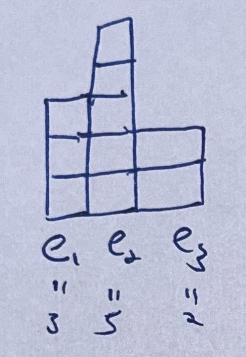
\includegraphics[width=0.15\textwidth]{./img/multi-1.png} 
        \end{figure}
        \item 按勒贝格积分思想,横着计算,第一步计算$g_2*g_2$,第二步计算$\alpha = g_2*g_1$,第三步计算$\beta = \alpha * g_3$,第四步计算$\gamma = \beta * \beta$,第五步计算$\beta * \alpha$, 第六步计算$(\beta * \alpha) * (g_2*g_2)$,总共进行6步乘法操作。
        \begin{figure}[H]
            \centering
            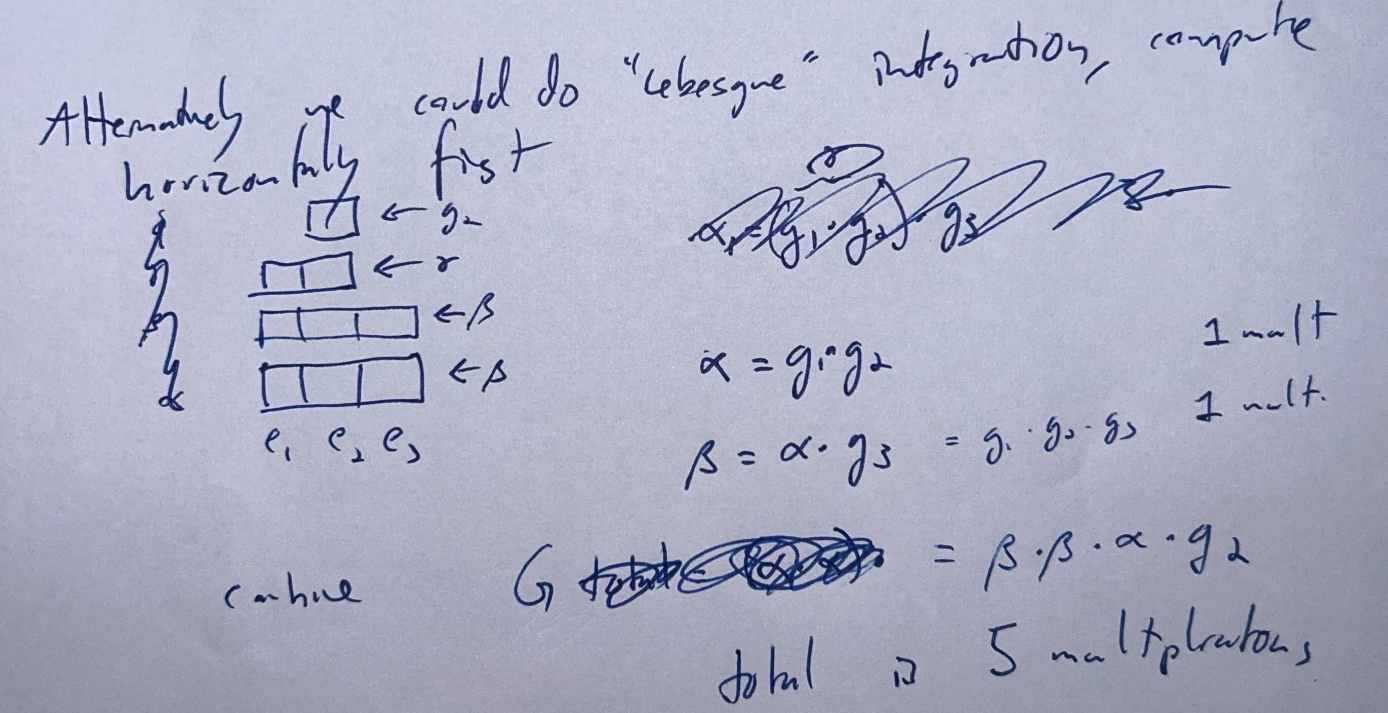
\includegraphics[width=0.9\textwidth]{./img/multi-2.png} 
        \end{figure}
    \end{itemize} 
\end{itemize}
计算$g_1^{2^k}g_2^{2^k} \cdots g_n^{2^k}=(g_1g_2 \cdots g_n)^{2^k}$,先计算括号里的乘积$g_1g_2 \cdots g_n$,也就是$n-1$次乘法,再将结果进行平方,$k$次平方,总共进行$n - 1 + k$次乘法操作。

假设$\mathbb{G}$是一个$p$阶循环群,其中$p$是一个$\lambda$-位素数,设$\lambda = 256$.计算
$$
G = \prod_{i = 0}^{N-1}g_i^{e_i},
$$
其中$e_i$是整数。假设$\lambda \ge N$并且将$\lambda$分解成$s$个legs,即$\lambda = s \cdot t$,例如$\lambda = 256, s=4$,$t=64$,$N=16$.(一般取$s \approx \sqrt{\frac{\lambda}{N}}$,且$t = \sqrt{\lambda N}$)

令$e_i = \sum_{l=0}^{\lambda - 1}e_{i,l} \cdot 2^l$($e_{i,l} \in \{0,1\}$,也就是将$e_i$写成二进制形式).将$\lambda$分解成$s$条legs,则
$$
e_i = \sum_{j=0}^{s-1} \sum_{k=0}^{t-1}e_{i,j+sk} \cdot 2^{j+sk}
$$
例如$\lambda = 256 = 4 \cdot 64$.
\begin{figure}[H]
    \centering
    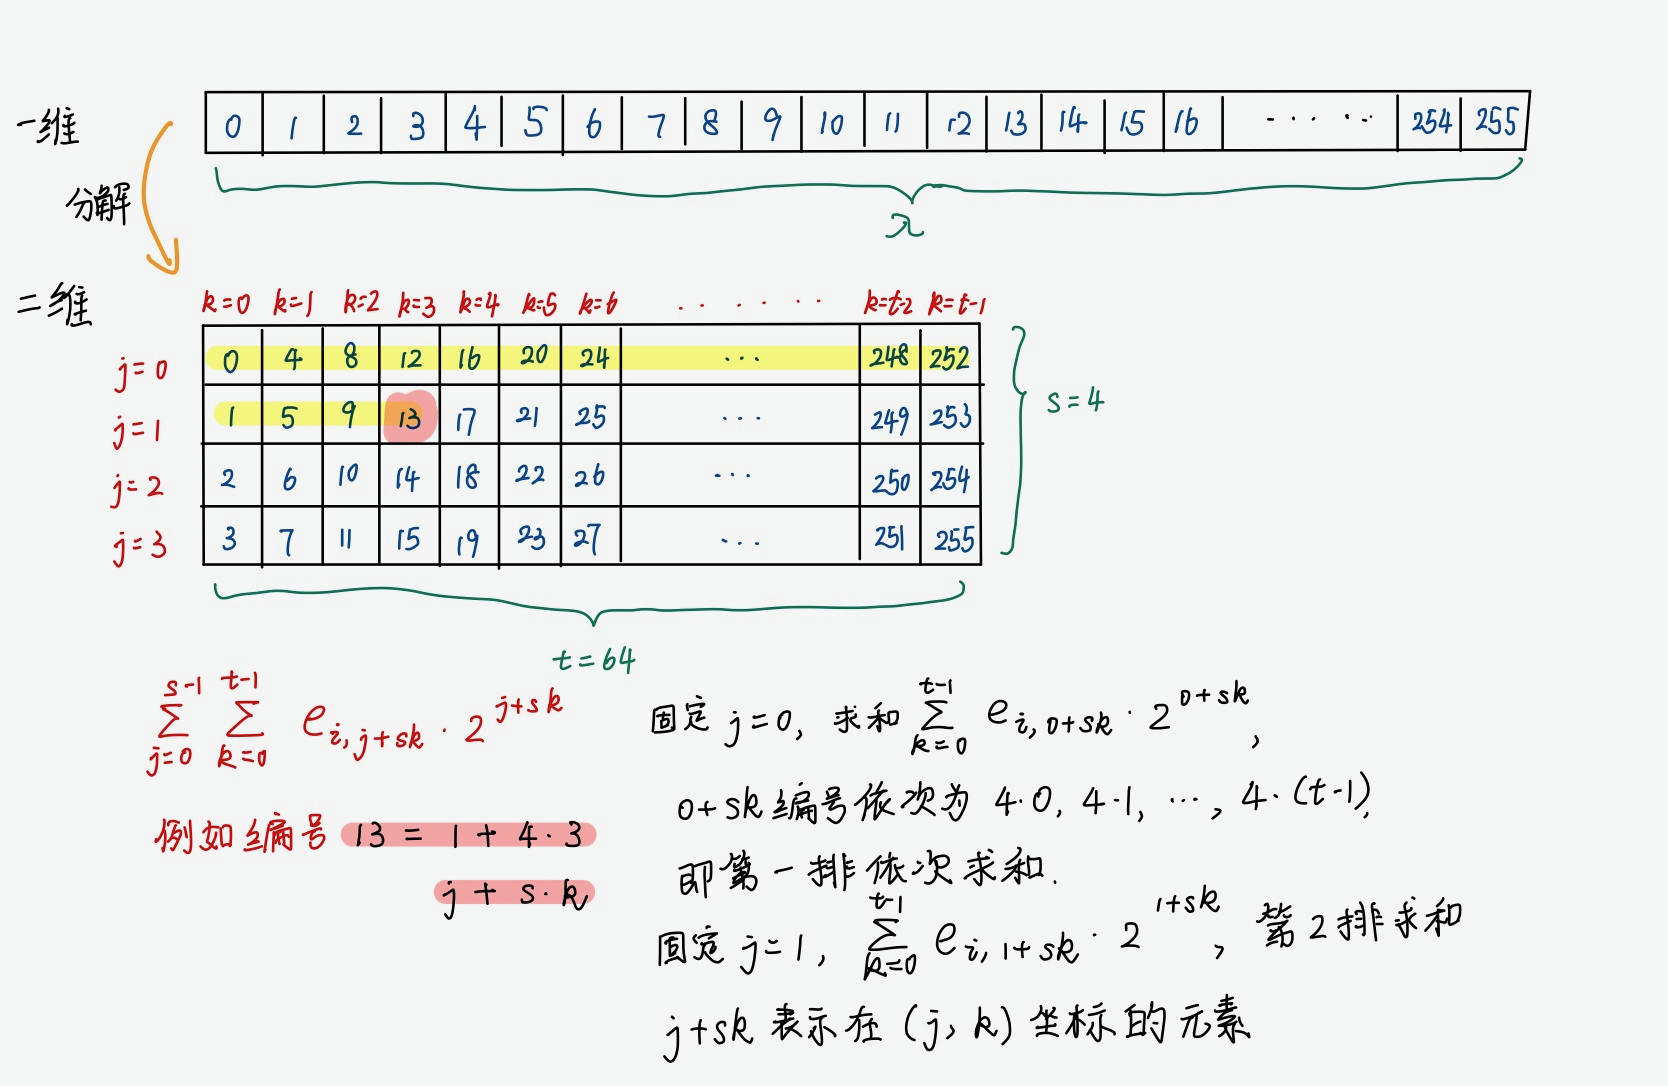
\includegraphics[width=1\textwidth]{./img/sum.png} 
\end{figure}
因此
$$
g_i^{e^i} = \prod_{l=0}^{\lambda -1}g_i^{2^l \cdot e_{i,l} } \overset{\lambda = s \cdot t}{=} \prod_{j=0}^{s-1} \prod_{k=0}^{t-1} g_i^{2^{j+sk} \cdot e_{i,j+sk}},
$$
接着计算$G$
\begin{displaymath}
    \begin{aligned}
        G= \prod_{i = 0}^{N-1}g_i^{e^i} & = \prod_{i = 0}^{N-1} \left( \prod_{j=0}^{s-1} \prod_{k=0}^{t-1} g_i^{2^{j+sk} \cdot e_{i,j+sk}} \right)\\
        & = \prod_{k = 0}^{t-1} \left( \prod_{i=0}^{N-1} \prod_{j=0}^{s-1}  g_i^{2^{j} \cdot e_{i,j+sk}} \right)^{2^{sk}}
    \end{aligned}
\end{displaymath}
记括号里
$$
G_k^{\prime} := \prod_{i=0}^{N-1} \prod_{j=0}^{s-1}  g_i^{2^{j} \cdot e_{i,j+sk}}.
$$
将每一个$i=0,1,\cdots,N-1$依次从上到下排列,最终的结构如下:
\begin{figure}[H]
    \centering
    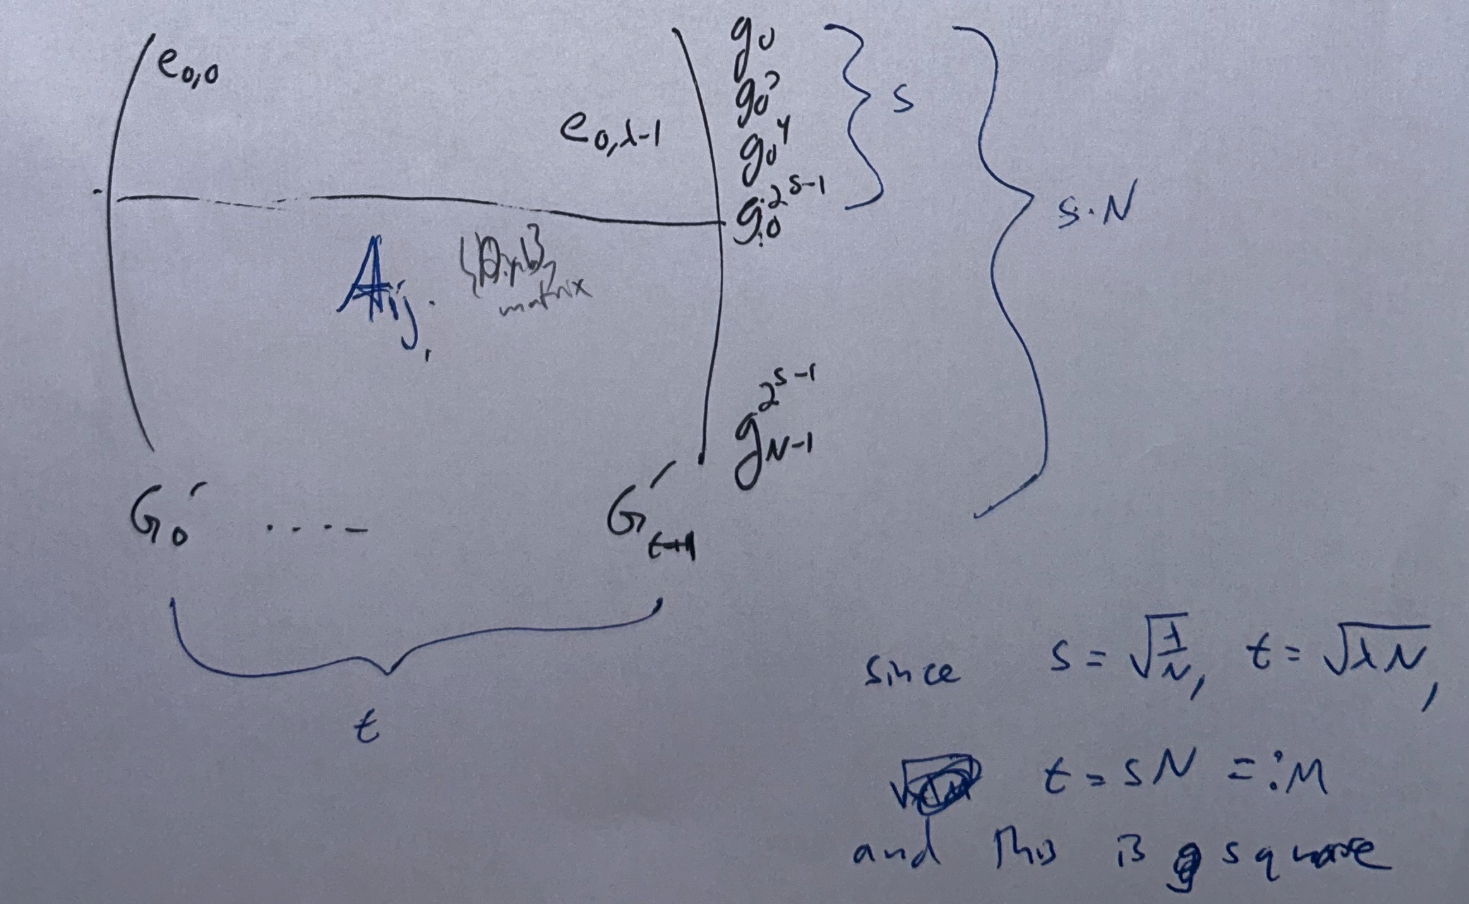
\includegraphics[width=1\textwidth]{./img/matrix.png} 
\end{figure}
每一个$G_k^{\prime}(k = 0, 1, \cdots t-1)$就是竖着的一整列。对于每一个$G_k^{\prime}$乘积内部$g_i^{2^{j} \cdot e_{i,j+sk}}$,需要计算下面这些项:
$$
g_i,g_i^2,g_i^4, \cdots, g_i^j, \cdots,g_i^{2^{s-1}}
$$
总共有$N$个这样的乘积$G_k^{\prime} := \prod_{i=0}^{N-1} \left(\prod_{j=0}^{s-1}  g_i^{2^{j} \cdot e_{i,j+sk}}\right)$,因此总的花销是$N * s = N * \sqrt{\lambda / N} = \sqrt{\lambda N}$.

更一般地,将列向量中的元素分成多个块,每块中至多有$b$个元素。如果列向量中总共有$M$个元素,则将列向量最终分为$S_0, \cdots, S_{\frac{M}{b}-1}$。对于每一个$S_i$,计算$S_i$中所有可能的乘积,记为$T_i$.例如$b=3$,则$S_0=\{h_0,h_1,h_2\},T_0=\{h_0,h_1,h_2,h_0h_1,h_0h_2,h_1h_2,h_0h_1h_2\}.$
\begin{itemize}
    \item 每个$S_i$中有$b$个元素,所有可能的乘积$T_i$中有$2^b$个元素。总共有$M/b$个集合,因此所有集合中乘积有$\frac{2^bM}{b}$个。
    \item 每列有$M/b$个$T_i$,有$M$列,总共有$\frac{M^2}{b}$个$T_i$.
    \item $G_k^{\prime}$中,列向量划分后,每个$S_i$中有$b=s$个元素,一列有$M = s \cdot N$个元素,有$M$列,设置$t = M = s \cdot N$,形成一个方阵。
\end{itemize}

刚刚计算了每个$G_k^{\prime}$,最后要计算
$$
G = \prod_{k = 0}^{t-1} (G_k^{\prime})^{2^{sk}}
$$
\begin{figure}[H]
    \centering
    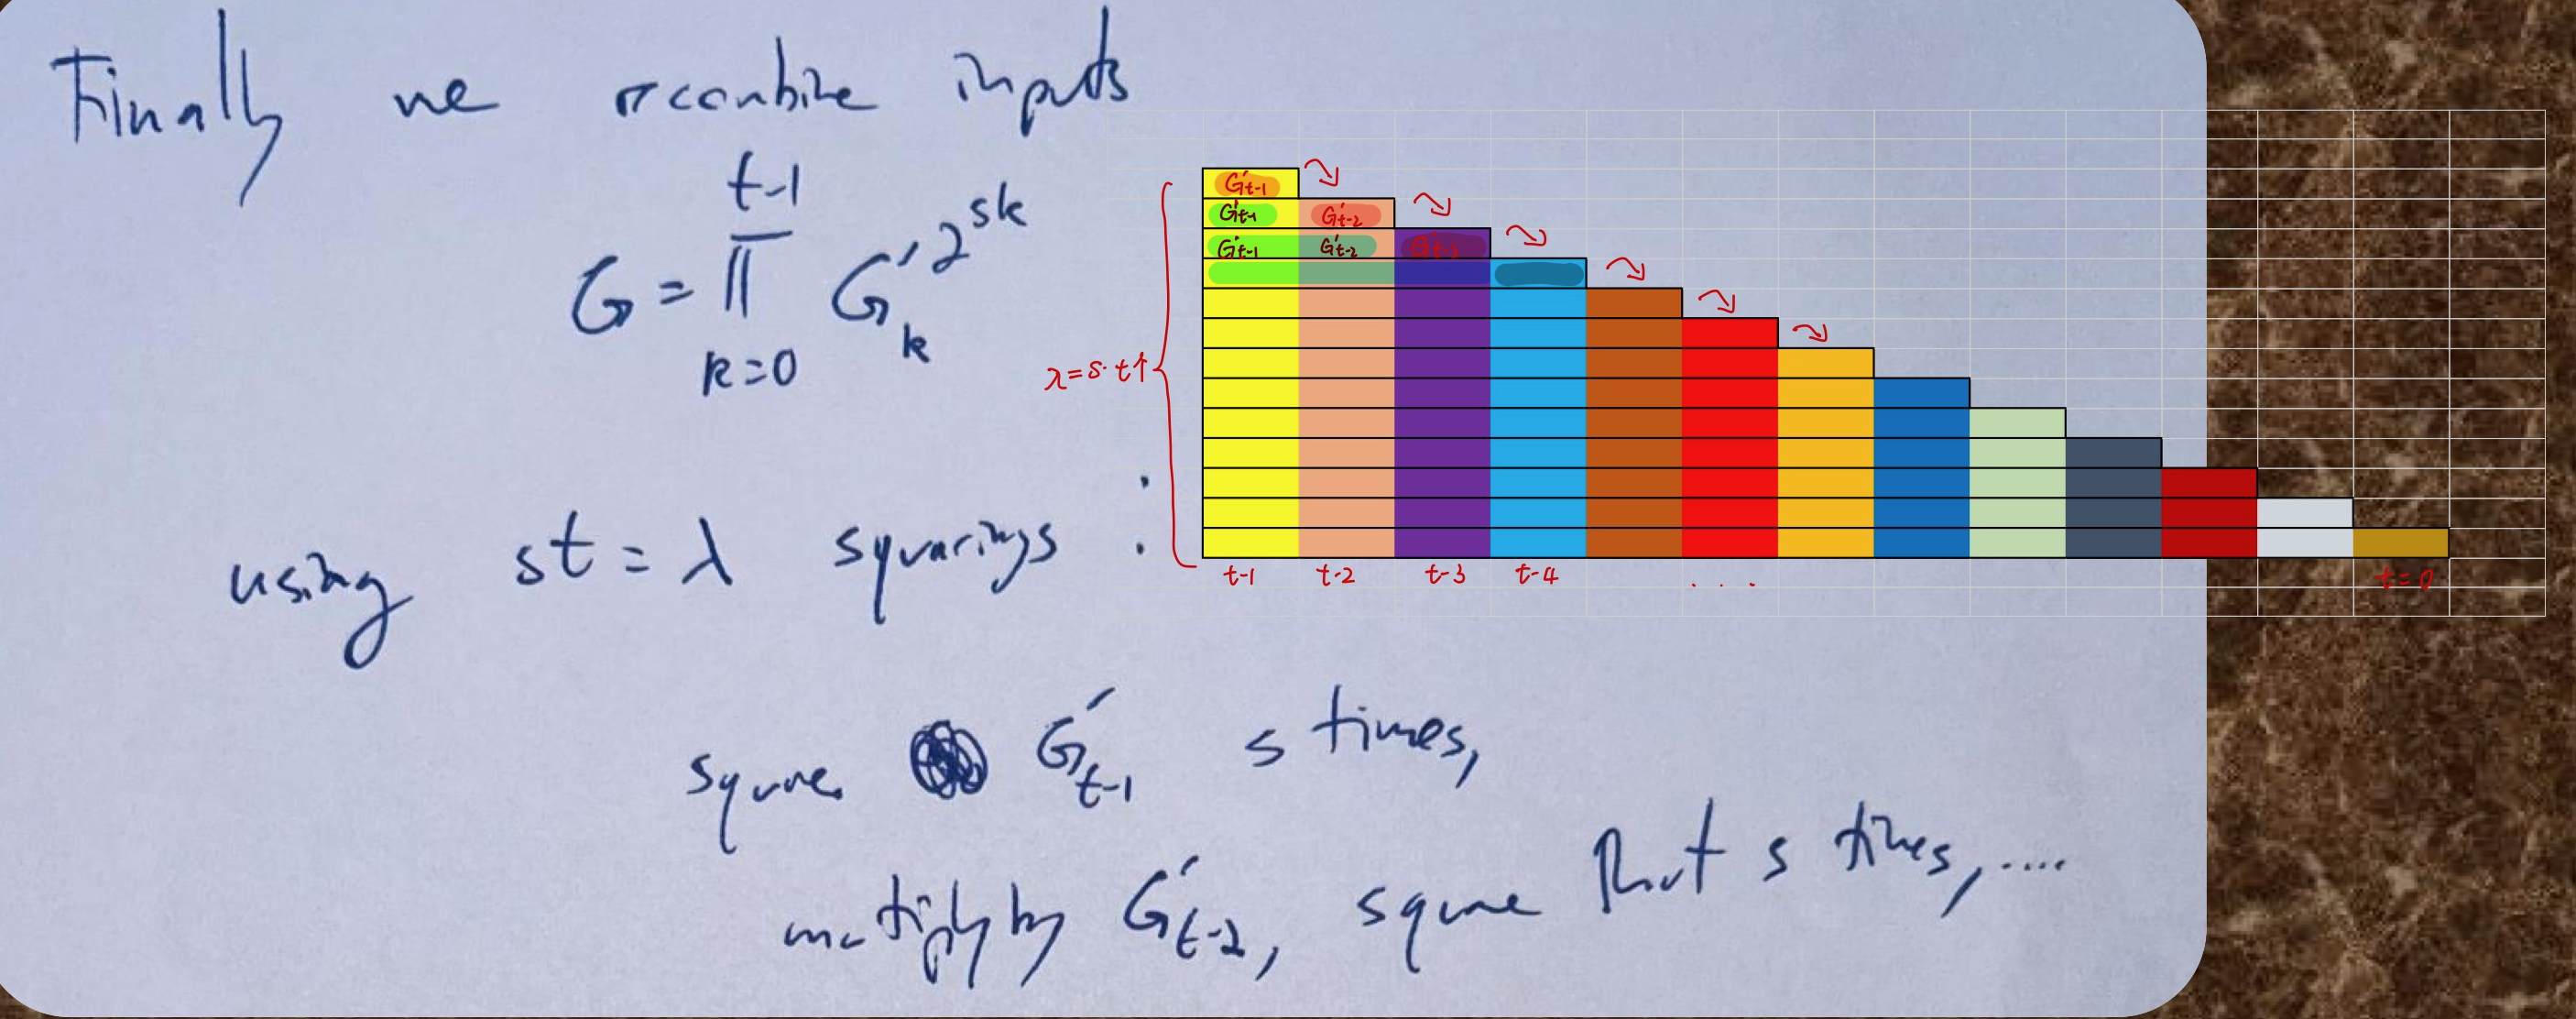
\includegraphics[width=1\textwidth]{./img/G.png} 
\end{figure}
计算$G = \prod_{k = 0}^{t-1} (G_k^{\prime})^{2^{sk}} = \prod_{k = 0}^{t-1} \left((G_k^{\prime})^{2^s}\right)^k$,具体为:
\begin{enumerate}
    \item $ans_{t - 1} = \left(G_{t-1}^{\prime}\right)^{2^s} * \left(G_{t-2}^{\prime}\right)^{2^s}$ 
    \item $ans_{t-2} = ans_{t - 1} * \left(G_{t-3}^{\prime}\right)^{2^s} = G_{t-1}^{\prime} * \left(G_{t-2}^{\prime}\right)^{2^s} * \left(G_{t-3}^{\prime}\right)^{2^s}$ 
    \item $ans_{t-3} = ans_{t - 2} * \left(G_{t-4}^{\prime}\right)^{2^s} = G_{t-1}^{\prime} * \left(G_{t-2}^{\prime}\right)^{2^s} * \left(G_{t-3}^{\prime}\right)^{2^s} * \left(G_{t-4}^{\prime}\right)^{2^s}$ 
    \item $\cdots$
    \item $ans_{1} = ans_{2} * \left(G_{0}^{\prime}\right)^{2^s} = G_{t-1}^{\prime} * \left(G_{t-2}^{\prime}\right)^{2^s} * \left(G_{t-3}^{\prime}\right)^{2^s} * \left(G_{t-4}^{\prime}\right)^{2^s} * \cdots * \left(G_{1}^{\prime}\right)^{2^s} * \left(G_{0}^{\prime}\right)^{2^s}$ 
    \item $G = ans_{t-1} * ans_{t-2} * \cdots * ans_{2} * ans_{1}$
\end{enumerate}
先对$G_{t-1}^{\prime}$进行$s$次平方操作,再乘以$\left(G_{t-2}^{\prime}\right)^{2^s}$,以此类推。这里每个$\left(G_{k}^{\prime}\right)^{2^s}$进行$s$次平方操作,总共有$t$个,因此进行$\lambda = s * t$次平方操作。总共有$t = M$次乘法操作\mnote{在上述第6步中要将乘法结果相乘,不应该是$t + (t - 1)$次乘法操作吗?}。

由于$M = \sqrt{\lambda N} = t = sN$,总共计算次数为:
\begin{figure}[H]
    \centering
    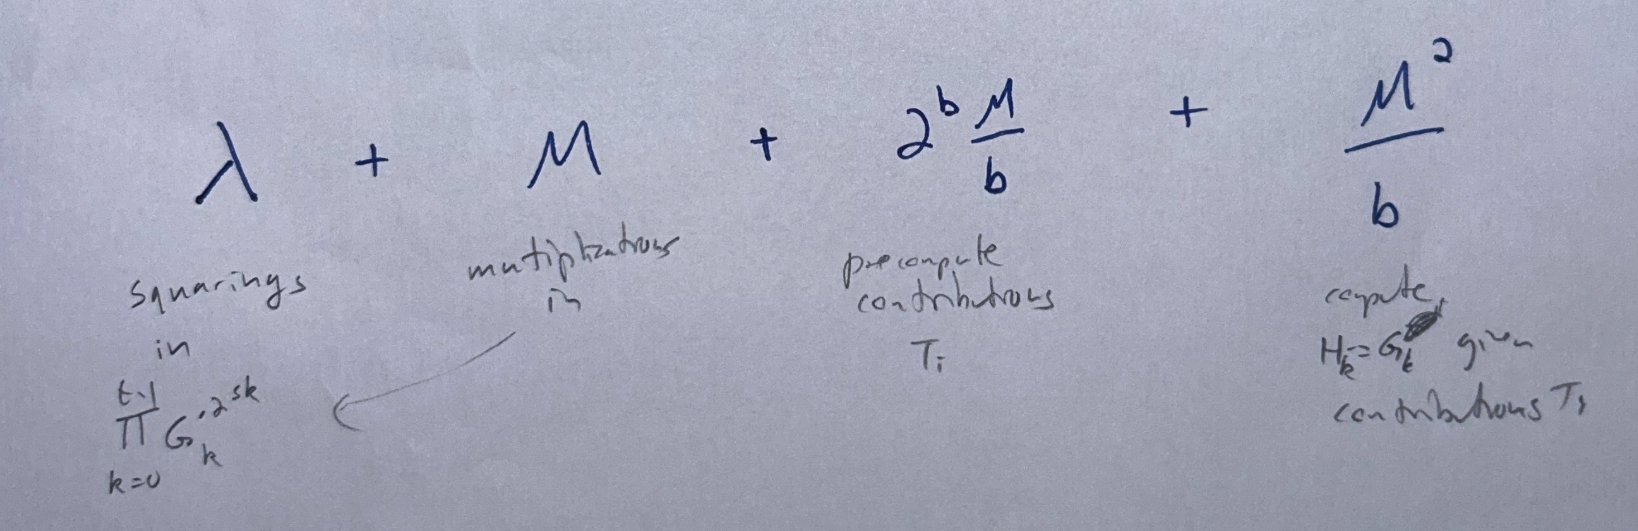
\includegraphics[width=1\textwidth]{./img/operates.png} 
\end{figure}
上述式子中$b$是参数,通过求极小值方法,确定$b$的最优值,即
$$
b = \log M - \log \log M,
$$
将$b$的值代入得
\begin{displaymath}
    \begin{aligned}
         & \lambda + M +  2^b \frac{M}{b} + \frac{M^2}{b} \\
         & \quad = \lambda + M +  2^b \frac{M^2}{\left(\log M - \log \log M\right)\left(\log M\right)} + \frac{M^2}{\log M - \log \log M} \\
         & \quad = \lambda + (1 + o(1))\frac{M^2}{\log M} \\
         & \quad = \lambda + (1 + o(1))\frac{\lambda N}{\log \lambda N} \quad \quad(M = t = \sqrt{\lambda N}).
    \end{aligned}
\end{displaymath}

\section{FFT \& DFT高效算法}
两种方式得到一个多项式$f(x)$:
\begin{enumerate}
    \item 得到多项式$f(x)$的各项系数,如$3+4x+7x^2+5x^3+\cdots$,或者多元多项式$3x_1x_7x_{10} + 11x_2x_7x_{8}+\cdots$.
    \item 在一些点处进行估值,如果多项式$f(x)$次数为degree,则需要在degree $+1$个不同的点进行估计。其实本质还是算出多项式的系数。
\end{enumerate}

\begin{theorem}
    假设$x_1,\cdots,x_p \in \mathbb{F}^m$是数域$\mathbb{F}^m$上不同的点,则下述是等价的:
    \begin{enumerate}
        \item[(1)] 给定$y_1,\cdots,y_p \in \mathbb{F}$,存在唯一的$f \in F[\vec{x}](deg_f \le n)$使得$f(x_i) = y_i \quad (\forall 1 \le i \le p)$.
        \item[(2)] $p \times p$矩阵
        $$
        M = \left(x_i^{I_j}\right)
        $$
        是可逆的。其中,$I_j$表示$x_i$对应的次数($0 \le I_j \le p - 1$)。该矩阵具体形式如下:
        \begin{displaymath}
            M =      \left(
            \begin{matrix}
                1 & x_1 & x_1^2 & \cdots & x_1^{p-1} \\
                1 & x_2 & x_2^2 & \cdots & x_2^{p-1} \\
                1 & x_3 & x_3^2 & \cdots & x_3^{p-1} \\
                \vdots & \vdots & \vdots &  & \vdots \\
                1 & x_p & x_p^2 & \cdots & x_p^{p-1} 
            \end{matrix}
        \right)
        \end{displaymath}
    \end{enumerate}
\end{theorem}
$p$级Vandermonde行列式$|M|$等于$x_1,x_2,\cdots,x_p$这$p$个数所有可能的差$x_i - x_j(1 \le i < j \le p)$的乘积,即
$$
|M| = \prod_{1 \le i < j \le p}(x_i - x_j).
$$
由于$x_1,x_2,\cdots x_p$各不相同,自然$|M| \neq 0$,因此矩阵$M$也是可逆的。

对于多项式的加法,假设
$$
f(x) = a_0 + a_1 x + a_2 x^2 + a_3 x^3,
$$
$$
g(x) = b_0 + b_1 x + b_2 x^2 + b_3 x^3.
$$
计算$f(x) + g(x)$:
\begin{itemize}
    \item 如果用系数表达方式,则只需要将各次数前的系数相加即可:
    $$
    f(x) + g(x) = (a_0 + b_0) + (a_1 + b_1)x + (a_2 + b_2)x^2 + (a_3 + b_3)x^3.
    $$
    如果多项式$f(x)$和$g(x)$的次数都是$deg = deg_f = deg_g$,则需要进行$deg + 1$次加法操作。
    \item 用估值方法,需要进行4次估值:
    \begin{displaymath}
        \begin{aligned}
            (f+g)(1) = f(1) + g(1) \\
            (f+g)(2) = f(2) + g(2) \\
            (f+g)(3) = f(3) + g(3) \\
            (f+g)(4) = f(4) + g(4)
        \end{aligned}
    \end{displaymath}
    一般地,也是需要估计$deg + 1$个点。
\end{itemize}

下面考虑多项式的乘法。例如
$$
f(x) = a_0 + a_1 x + a_2 x^2,
$$
$$
g(x) = b_0 + b_1 x + b_2 x^2 + b_3 x^3.
$$
自然$f(x)g(x)$需要进行$(deg_f + 1)(def_g + 1)$次乘法操作。此例中
\begin{displaymath}
    \begin{aligned}
        f \cdot g & = (a_0 + a_1 x + a_2 x^2)(b_0 + b_1 x + b_2 x^2 + b_3 x^3) \\
        & = a_0b_0 + (a_0b_1 + a_1 b_0)x + (a_0b_2 + a_1 b_1 + a_2 b_0)x^2 + \cdots
    \end{aligned}
\end{displaymath}
一般地,
$$
(f \cdot g)_l = \sum_{j + k = l} a_j b_k =  \sum_{j=0}^l a_j b_{l-j}.
$$
用系数表示的方式求$f \cdot g$就需要进行$(deg_f + 1)(def_g + 1)$次操作,如果$f,g$都是$n$次多项式,计算就需要$O(n^2)$.

但是观察到其实$f \cdot g$乘积多项式的次数只有$deg_f + deg_g$,也就是说如果用点估值的方式,只需要进行估计$deg_f + deg_g + 1$个点,这样的计算量远小于系数表达方式的$(deg_f + 1)(def_g + 1)$.如果$f,g$都是$n$次多项式,计算量就是$O(n)$了。究竟找哪$2n + 2$个点进行估值呢?估值后的结果如何逆向算出原来的多项式呢?

对于一般的$n-1$次多项式$f(x) = a_0 + a_1 x + a_2 x^2 + \cdots + a_{n-1} x^{n-1}$,得到不同的$n$个点$x_i$的估值$f(x_i) = y_i$后,可以得到
\begin{displaymath}
    \begin{aligned}
        f(x_0) = a_0 + a_1 x_0 + a_2 x_0^2 & + \cdots + a_{n-1} x_0^{n-1} = y_0 \\
        f(x_1) = a_0 + a_1 x_1 + a_2 x_1^2 & + \cdots + a_{n-1} x_1^{n-1} = y_1 \\
        & \vdots \\
        f(x_{n-1}) = a_0 + a_1 x_{n-1} + a_2 x_{n-1}^2 & + \cdots + a_{n-1} x_{n-1}^{n-1} = y_{n-1}
    \end{aligned}
\end{displaymath}
目的是要求出$a_0,a_1,\cdots, a_{n-1}$,上述方程组可以写为:
\begin{displaymath}
    \left(
    \begin{matrix}
        1 & x_0 & \cdots & x_0^{n-1} \\
        1 & x_1 & \cdots & x_1^{n-1} \\
        1 & x_2 & \cdots & x_2^{n-1} \\
        \vdots & \vdots & & \vdots \\
        1 & x_{n-1} & \cdots & x_{n-1}^{n-1} 
    \end{matrix}\right)
    \left(\begin{matrix}
        a_0 \\
        a_1 \\
        a_2 \\
        \vdots \\
        a_{n-1}
    \end{matrix}\right)
    = \left(\begin{matrix}
        y_0 \\
        y_1 \\
        y_2 \\
        \vdots \\
        y_{n-1}
    \end{matrix}\right)
\end{displaymath}
注意上面矩阵形式,容易发现左侧矩阵就是Vandermonde矩阵$M$。记未知向量$\vec{a} = (a_0, a_1, \cdots, a_{n-1})^{\intercal}$,右端向量$\vec{y} =(y_0,y_1,\cdots, y_{n-1})^{\intercal}$,则上述方程组可写为:
$$
M\vec{a}=\vec{y}.
$$
上述方程的解为$\vec{a} = M^{-1} \vec{y}$.经过现在的分析,估值法求解一般$n-1$次多项式$f$(特别地就是前面想计算的$f \cdot g$)要解决的关键问题就是:
\begin{itemize}
    \item {\color{red}如何选取适当的估值点使得Vandermonde矩阵的逆容易计算?}
    
    {\color{blue}(选取素$n$次单位根$1, \omega, \omega^2, \cdots, \omega^{n-1}$, 这样$M^{-1} = (V_{\omega})^{-1} = \frac{1}{n} V_{\omega^{-1}} $)}

    \item {\color{red}如何能快速计算函数$f$在这些估计点的值$f(x_i)$呢?}{\color{blue}(离散傅里叶变换DFT)}
\end{itemize}


为了解决上述问题,将实数域上的问题考虑在复数空间去解决。引入复数域中的单位根。
\begin{itemize}
    \item $n$次单位根$\omega^n = 1$.
    \item 素$n$次单位根$\omega$就是,对任意的自然数$q < n$,有$\omega^q \neq 1$.
\end{itemize}
实数域上之前是用$f(1),f(2),\cdots$来进行估值,现在替换成用素单位根$f(\omega^1),f(\omega^2),\cdots$来进行估值。

如果$f = \sum_{j=0}^{n-1}f_jx^j$是一个多项式,系数为$f_0,\cdots,f_{n-1}$,需要做的就是一个映射$DFT_{\omega}:\mathbb{F}_q^n \rightarrow \mathbb{F}_q^n$
$$
f \mapsto (f(1), f(\omega),f(\omega^2), \cdots, f(\omega^{n-1}))
$$
这个就是离散傅里叶变换(Discrete Fourier Transform, DFT)。

对于多项式$f$与$g$
\begin{displaymath}
    \begin{aligned}
        f=f_0 + f_1 x + \cdots + f_{n-1}x^{n-1}\\
        g=g_0 + g_1 x + \cdots + g_{n-1}x^{n-1}
    \end{aligned}
\end{displaymath}
定义一个模$n$的卷积
\begin{displaymath}
    h = f *_n g = \sum_{l=0}^{n-1} h_l x^l,\quad h_l = \sum_{j+k= l \mod n}f_jg_k
\end{displaymath}
特别地,如果$0 \le l < n$, 那么$h_l = \sum_{j=0}^{n-1}f_jg_{l-j}$.

\begin{example}
    \begin{displaymath}
        \begin{aligned}
            \quad & {\color{blue} 2x^6+3x^5+x^4}+{\color{red} 3x^3 + 3x^2 + x + 1} \mod x^4 - 1 \\
            = & {\color{blue} (2x^2+3x+1)(x^4-1) + (2x^2 + 3x + 1)}+{\color{red} 3x^3 + 3x^2 + x + 1} \mod x^4 - 1\\
            & (\text{由于第一项能够整数,因此}{\color{blue} (2x^2+3x+1)(x^4-1)} \mod x^4 - 1 = 0) \\
            = & {\color{blue} (2x^2 + 3x + 1)}+{\color{red} 3x^3 + 3x^2 + x + 1} \mod x^4 - 1 \\
            = & 3x^3 + 5x^2 + 4x + 1 \mod x^4 - 1
        \end{aligned}
    \end{displaymath}
\end{example}

$*_n$是循环卷积,等价于在$\frac{\mathbb{F}_q[x]}{(x^n-1)}$(实际上是商群)中的多项式乘法
$$
f * g \equiv fg \mod x^n - 1.
$$
如果$deg(fg)<n$,那么$f * g = fg \mod x^n - 1$意味着$fg = f * g$.

找到的$n$使得$k \approx \log_2 n$, DFT方法计算是$O(n \log_2n)$.
\begin{figure}[H]
    \centering
    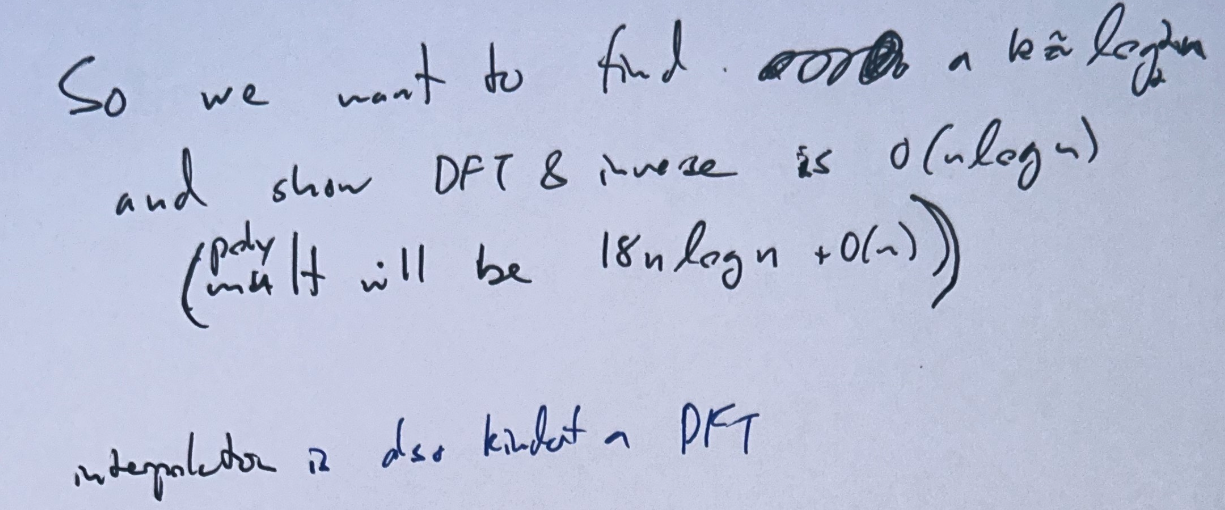
\includegraphics[width=1\textwidth]{./img/DFT.png} 
\end{figure}
Vandermonde矩阵
\begin{displaymath}
    V_{\omega} =      \left(
    \begin{matrix}
        1 & 1 & 1 & \cdots & 1 \\
        1 & \omega & \omega^2 & \cdots & \omega^{n-1} \\
        1 & \omega^2 & \omega^4 & \cdots & \omega^{2(n-1)} \\
        \vdots & \vdots & \vdots &  & \vdots \\
        1 & \omega^{n-1} & \omega^{2(n-1)} & \cdots & \omega^{(n-1)^2} 
    \end{matrix}
\right)
    = \left(\omega^{jk}\right), \quad 0 \le j,k <n.
\end{displaymath}
$V_{\omega}$是可逆的,$(V_{\omega})^{-1} = \frac{1}{n}V_{\omega^{-1}}$, $\omega^{-1}$也是单位根,$V_{\omega^{-1}}$是比较容易计算的,因此容易计算出$(V_{\omega})^{-1}$.

$n$是偶数(通常取$n=2^k$),$\omega$是素$n$次单位根,$f$的次数$deg < n$.为了估计$f$在$1,\omega,\omega^2,\cdots,\omega^{n-1}$的值,将$f$分别除以$x^{n/2}-1$和$x^{n/2}+1$, 余项记为$r_i$.
\begin{displaymath}
    f = q_0(x^{n/2}-1) + r_0 = q_1(x^{n/2}+1) + r_1, \quad q_0,r_0,q_1,r_1 \in \mathbb{F}[x], deg < n/2.
\end{displaymath}
这样商和余数多项式的次数就至少减半了。由于$0 = \omega^n - 1 = (\omega^{n/2} - 1)(\omega^{n/2} + 1)$, $\omega$是素单位根,因此$\omega^{n/2} - 1 \neq 0$, 那么$\omega^{n/2} + 1 = 0$.对于$0 \le l < n/2$,
\begin{displaymath}
    \begin{aligned}
        & f(\omega^{2l}) = q_0(\omega^{2l})(\omega^{nl} - 1) + r_0(\omega^{2l}) = r_0(\omega^{2l}), \\
        & f(\omega^{2l+1}) = q_1(\omega^{2l+1})(\omega^{nl}\omega^{n/2} + 1) + r_1(\omega^{2l+1}) = r_1(\omega^{2l+1}).
    \end{aligned}
\end{displaymath}
即
\begin{displaymath}
    \begin{aligned}
        & f(\omega^{2l})  = r_0(\omega^{2l}), \\
        & f(\omega^{2l+1}) =  r_1(\omega^{2l+1}) = r_1(\omega (\omega^{2l})).
    \end{aligned}
\end{displaymath}
由于$r_0,r_1$的次数$degree < n/2$以及$\omega^2$是素$n/2$次单位根(因为$(\omega^2)^{n/2} = 1$),因此可以继续类似地进行上述步骤。

这样要估计多项式$f$在$1, \omega, \omega^2, \cdots, \omega^{n-1}$点处的值,只需要计算这些点在对应的$r_0$, $r_1$处的值就行了。那么余项$r_0$, $r_1$的表达式怎么计算呢?由于
\begin{displaymath}
    f = q_0(x^{n/2}-1) + r_0 = q_1(x^{n/2}+1) + r_1, \quad q_0,r_0,q_1,r_1 \in \mathbb{F}[x], deg < n/2.
\end{displaymath}
设$f = \sum_{j = 0}^{n-1}f_j x^j$,则
\begin{displaymath}
    \begin{aligned}
        r_0  & = f_0 + f_1x + \cdots + f_{n-1}x^{n-1} \mod x^{\frac{n}{2}} - 1 \\
        & = f_0 + f_1x + \cdots + f_{\frac{n}{2}}x^{\frac{n}{2}} + f_{\frac{n}{2} + 1}x^{\frac{n}{2} + 1} + \cdots + f_{n-1}x^{n-1}  \mod x^{\frac{n}{2}} - 1 \\
        & = f_0 +  \cdots + f_{\frac{n}{2}-1}x^{\frac{n}{2}-1} + (f_{\frac{n}{2}} + f_{\frac{n}{2} + 1}x + \cdots + f_{n-1}x^{n-1 - \frac{n}{2}})(x^{\frac{n}{2}} - 1) \\
        & \quad + f_{\frac{n}{2}} + f_{\frac{n}{2} + 1}x + \cdots + f_{n-1}x^{n-1 - \frac{n}{2}} \mod x^{\frac{n}{2}} - 1 \\
        & = f_0 + f_{\frac{n}{2}} + (f_1 + f_{\frac{n}{2} + 1})x + \cdots + (f_{\frac{n}{2}-1} + f_{n-1})x^{\frac{n}{2}-1} \mod x^{\frac{n}{2}} - 1 \\
        & = \sum_{0 \le j < \frac{n}{2}}(f_j + f_{j+\frac{n}{2}})x^j,
    \end{aligned}
\end{displaymath}
\begin{displaymath}
    \begin{aligned}
        r_1  & = f_0 + f_1x + \cdots + f_{n-1}x^{n-1} \mod x^{\frac{n}{2}} + 1 \\
        & = f_0 + f_1x + \cdots + f_{\frac{n}{2}}x^{\frac{n}{2}} + f_{\frac{n}{2} + 1}x^{\frac{n}{2} + 1} + \cdots + f_{n-1}x^{n-1}  \mod x^{\frac{n}{2}} + 1 \\
        & = f_0 +  \cdots + f_{\frac{n}{2}-1}x^{\frac{n}{2}-1} + (f_{\frac{n}{2}} + f_{\frac{n}{2} + 1}x + \cdots + f_{n-1}x^{n-1 - \frac{n}{2}})(x^{\frac{n}{2}} + 1) \\
        & \quad -( f_{\frac{n}{2}} + f_{\frac{n}{2} + 1}x + \cdots + f_{n-1}x^{n-1 - \frac{n}{2}}) \mod x^{\frac{n}{2}} - 1 \\
        & = f_0 - f_{\frac{n}{2}} + (f_1 - f_{\frac{n}{2} + 1})x + \cdots + (f_{\frac{n}{2}-1} - f_{n-1})x^{\frac{n}{2}-1} \mod x^{\frac{n}{2}} + 1 \\
        & = \sum_{0 \le j < \frac{n}{2}}(f_j - f_{j+\frac{n}{2}})x^j,
    \end{aligned}
\end{displaymath}

{\color{red}FFT算法}

输入: $n = 2^k$, $f = \sum_{j = 0}^{n-1}f_j x^j$, $\omega, \omega^2, \cdots, \omega^{n-1}$是单位元的素$n$次根。

输出:$DFT_{\omega}(f)  = (f(1), f(\omega),f(\omega^2), \cdots, f(\omega^{n-1})) \in \mathbb{F}_q^n$
\begin{enumerate}
    \item 如果$n=1$,返回$f_0$.
    \item 
    \begin{displaymath}
        \begin{aligned}
            & r_0 \leftarrow \sum_{0 \le j < \frac{n}{2}}(f_j + f_{j+\frac{n}{2}})x^j, \\
            & r_1^* \leftarrow \sum_{0 \le j < \frac{n}{2}}(f_j - f_{j+\frac{n}{2}})\omega^j x^j, \quad r_1^* = r_1(\omega x)
        \end{aligned}       
    \end{displaymath}
    \item 继续在$\omega^2$处估计$r_0$和$r_1^*$.
    \item 返回
    $$
    r_0(1),r_1^*(1),r_0(\omega^2),r_1(\omega^2), \cdots, r_0(\omega^{n-1}),r_1(\omega^{n-1}).
    $$
\end{enumerate}
在$\mathbb{F}$中进行$n\log_2n$次加法运算(每次$r_0$与$r_1^*$都需要进行加法,总共n次),$\frac{n}{2}\log_2n$次乘法运算(每次$r_1^*$中需要1次乘法,总共$n/2$次),因此总的域上计算操作是$\frac{3}{2}n\log_2n$次。

\end{document}